\section{Stability and Performance Analysis}

\subsection{Basic System Classes}

\subsubsection{First Order Systems}
State-space representation of first order system:
$$\dot{x} = -\frac{1}{\tau}x+\frac{k}{\tau}u$$
$$y=x$$

A first-order system has one  pole and is described by:
$$H(s)=\frac{k}{\tau s+1}$$
Where \emph{k} is the DC-gain and $\tau$ is the time-constant. The system has a pole
in $s=-\frac{1}{\tau}$ i.e., the smaller time-constant, the faster system response.


\subsubsection{Second Order Systems}
The transfer funciton of a second-order system is given by:
$$H(s) = \frac{k \omega_n^2}{s^2+2\zeta\omega_n s+\omega_n^2}$$
Where $\omega_n>0$ is the natural frequency and $\zeta>0$ is the damping ratio and k is the gain.

The system has two poles, which are $s\in \mathbb{C}$ where:
$$s^2+2\zeta\omega_n s+\omega_n^2=0$$
The values of s is given by:
$$s = -\zeta\omega_n \pm j\omega_n\sqrt{1-\zeta^2}$$

When $\zeta=1$ the system is critically damped and $H(s)$ has a double pole in $s=-\zeta \omega_n$,
when $0<\zeta<1$ the system is underdamped and has complex poles.
When $\zeta>1$ the system is overdamped and has real and distinct poles.

\begin{center}
	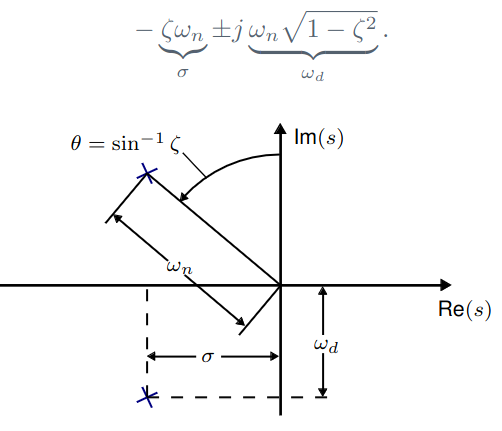
\includegraphics[width=0.5\textwidth]{Images/secondOrderSystem.png}
\end{center}

\newpage
Impulse response of a underdamped second-order system:
$$h(t) = k \frac{\omega_n}{\sqrt{1-\zeta ^2}} e^{-\sigma t} sin(\omega_d t) 1(t) $$

The step resonse of a underdamped second-order system:
$$y(t) = k(1-e^{-\sigma t}(\cos(\omega_d t)+\frac{\sigma}{\omega_d}\sin(\omega_d t)))$$

Impulse response of a critically damped second order system:
$$h(t) = k\omega_n^2te^{-\omega_n t}$$

Having a overdamped system with a damping ration that is greater than one leads to a slower impulse response.

The step response of a critically damped second order system:
$$y(t) = k(1-e^{-\omega_nt}-\omega_n te^{-\omega_nt})$$

Looking at the bode plot of a second-order system depends on the damping ratio.
For every pole the magnitude of the bode plot decreases by 20dB/decade.
And the phase of the bode plot decreases by 90 degrees for every pole.

\begin{center}
	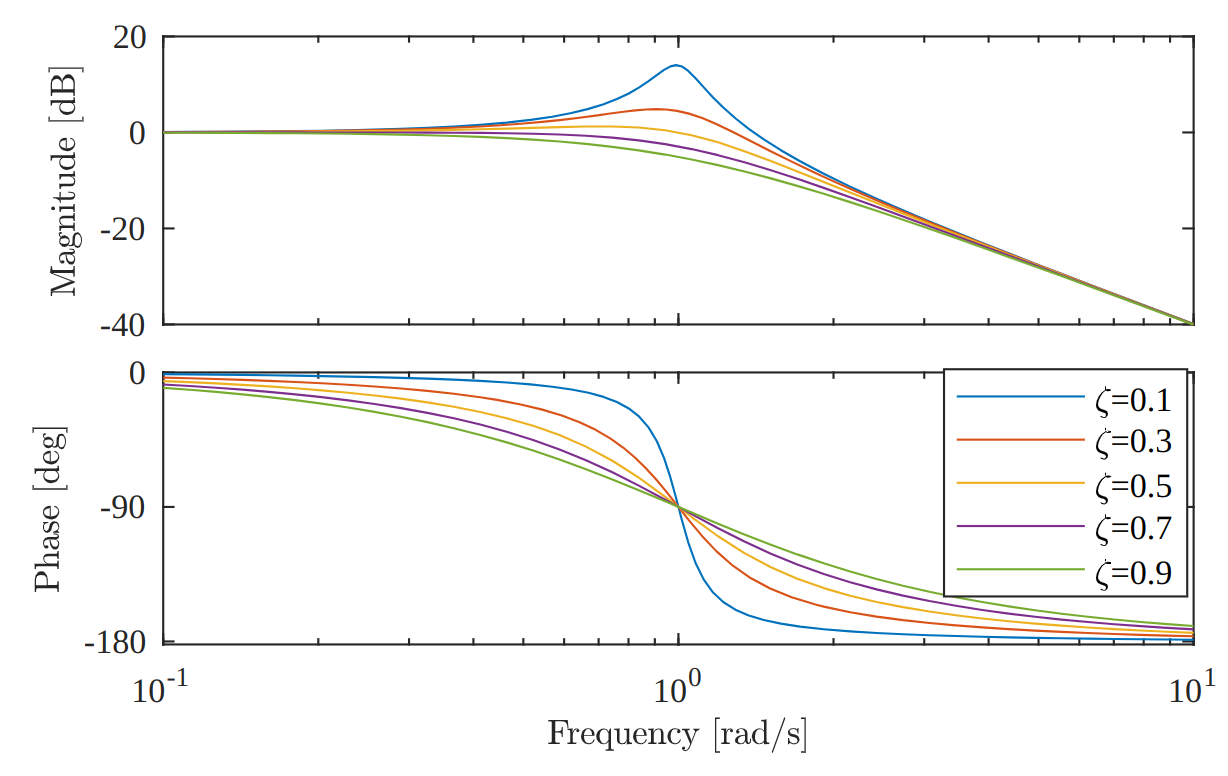
\includegraphics[width=0.5\textwidth]{Images/bodeSec.png}
\end{center}


\subsection{Performance specifications}

Three different performance measurements of dynamical systems are:
\begin{enumerate}
	\item{The rise time $t_r$ (stigetid)}
	\item{The settling time $t_s$ (indsvingingstid)}
	\item{The overshoot $M_p$ (oversving)}
\end{enumerate}

The rise time is the time it takes for the system to go from 10\% to 90\% of the final value.
The settling time is the time it takes for the system to reach and stay within a certain \% of the final value.
The overshoot is the maximum percentage that the system goes over the final value.

\begin{center}
	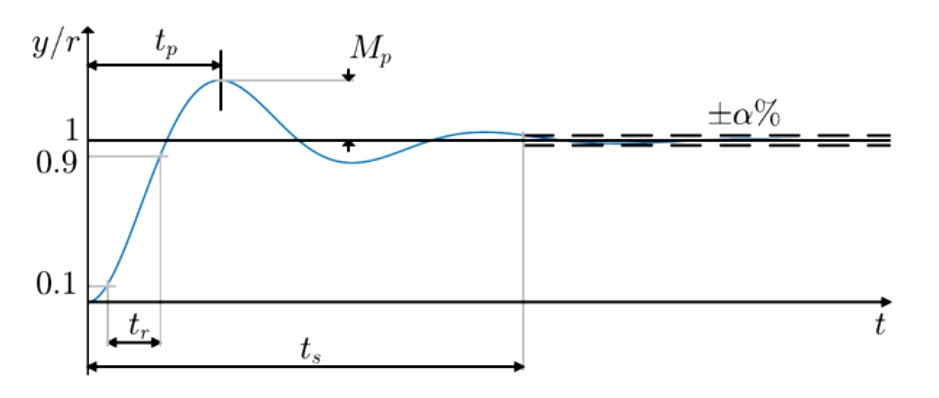
\includegraphics[width=0.5\textwidth]{Images/performance.png}
\end{center}

The peak time is denoted $t_p$ which is the time where the signal reaches its maximum value.

For a second-order system the rise time can be approximated as:
$$t_r = \frac{1.8}{\omega_n}$$

For a second-order system the settling time can be approximated as:
$$t_s = \frac{-log(\alpha/100)}{\zeta \omega_n}$$
Log is ln in the equation.

The peak time can be found using:
$$t_p = \frac{\pi}{\omega_d}$$

The overshoot is computed from the step response at the peak time. This gives
an expression for the overshoot:
$$M_p = e^{-\frac{\zeta \pi}{\sqrt{1-\zeta^2}}}$$
for $0<\zeta<1$. The overshoot is given in percentage.


\textbf{Overview for determining performance variables}
\begin{center}
	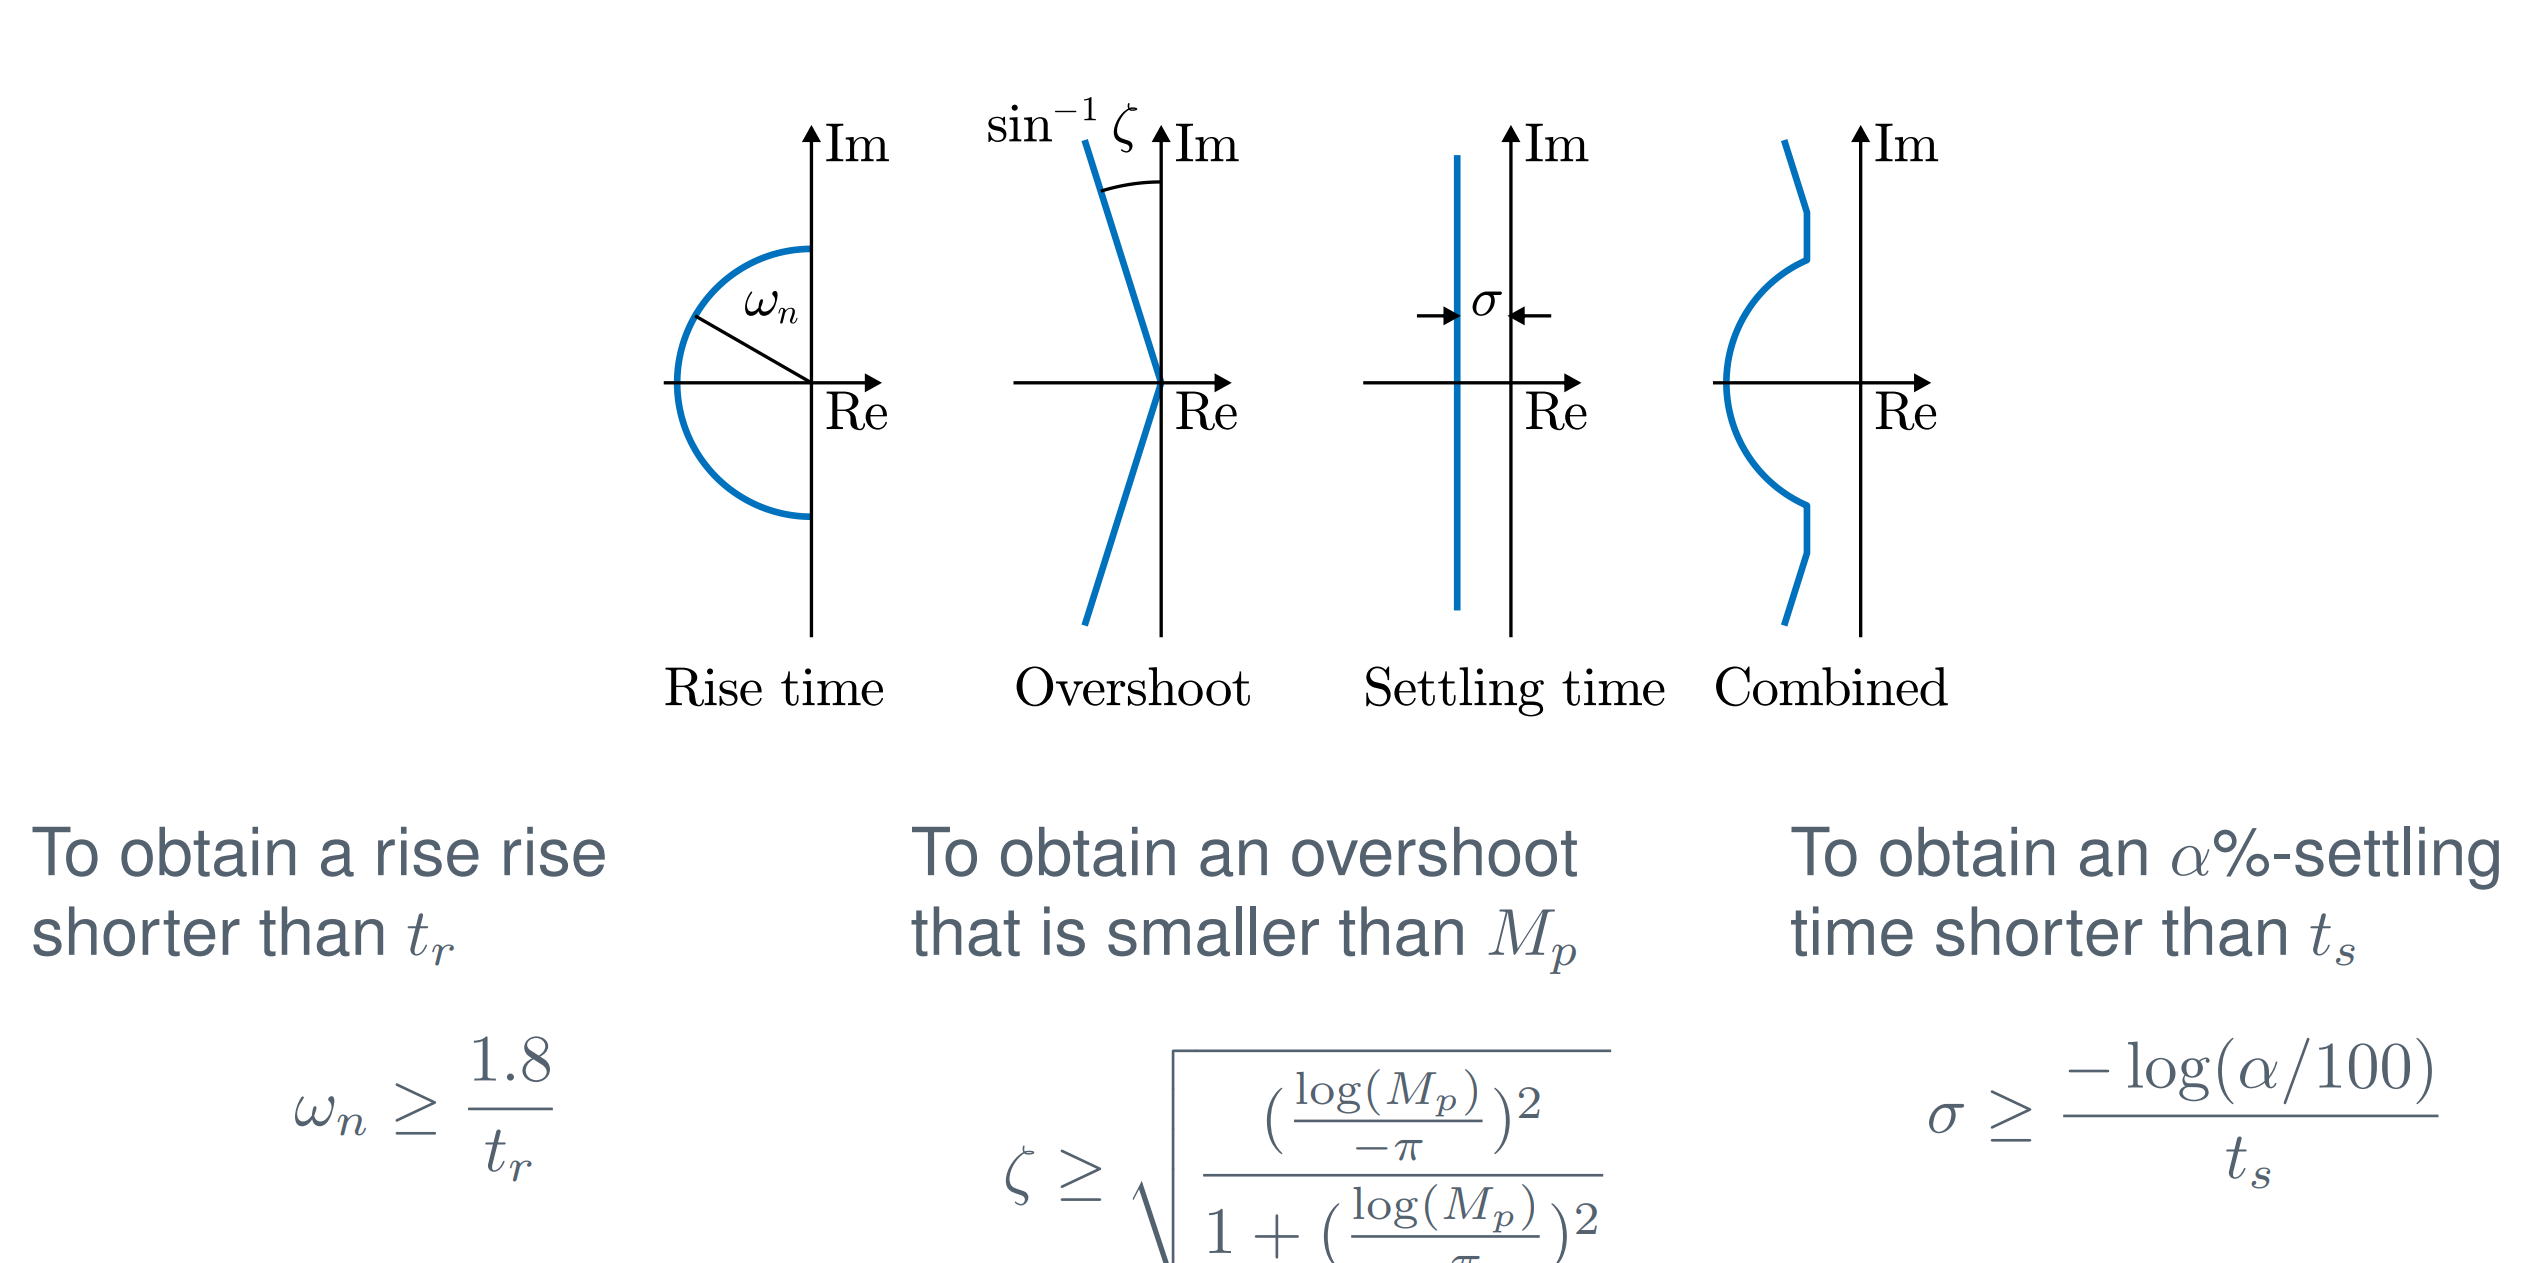
\includegraphics[width=\textwidth]{Images/perfSpec.png}
\end{center}


\subsection{Poles and Zeros of Space-State Models}
Using thee state-space matrices:
$$G(s) = C(sI-A)^{-1}B+D$$
\textbf{Poles} can be found using the following equation:

When $G(s)\to \infty$ the system has a pole at $s\to p$.
$$\det(pI-A) = 0$$
Here $p$ is the eigenvalue of $A$.

\textbf{Zeros} can be found using the following equation:

When $G(s)=0$ the system has a zero at $s=z$.
$$\begin{vmatrix}
		A-zI & B \\
		C    & D
	\end{vmatrix} = 0$$

Another definition of z being a zero for G(s) is when the matrix does not have full column rank.


\subsection{Stability}
The stability of the dynamical system can be determined from the eigenvalues of A in the time domain.
This is the equivalent of poles in the frequency domain.
$$\dot{x} = Ax+Bu$$
When the eigenvalues of A have a negative real part, the system is stable.

\textbf{Definition}
A linear discrete-time system
$$x_{k+1}=\Phi x_k$$
The state of the next time step is given by $\phi$ mutliplied by $x_k$.

Where $x_k \in \mathbb{R}^{n \times n}$ is asymptotically (asymptotisk) stable if
$$\lim_{k \to \infty} x_k = 0$$
for any $x_0 \in \mathbb{R}^n$.

A linear discrete-time system is stable if all the eigenvalues are inside the unit circle.


The closer the poles are to origin the more dominating the pole is in the system.


\subsection{Examples}
